\begin{figure*}
  %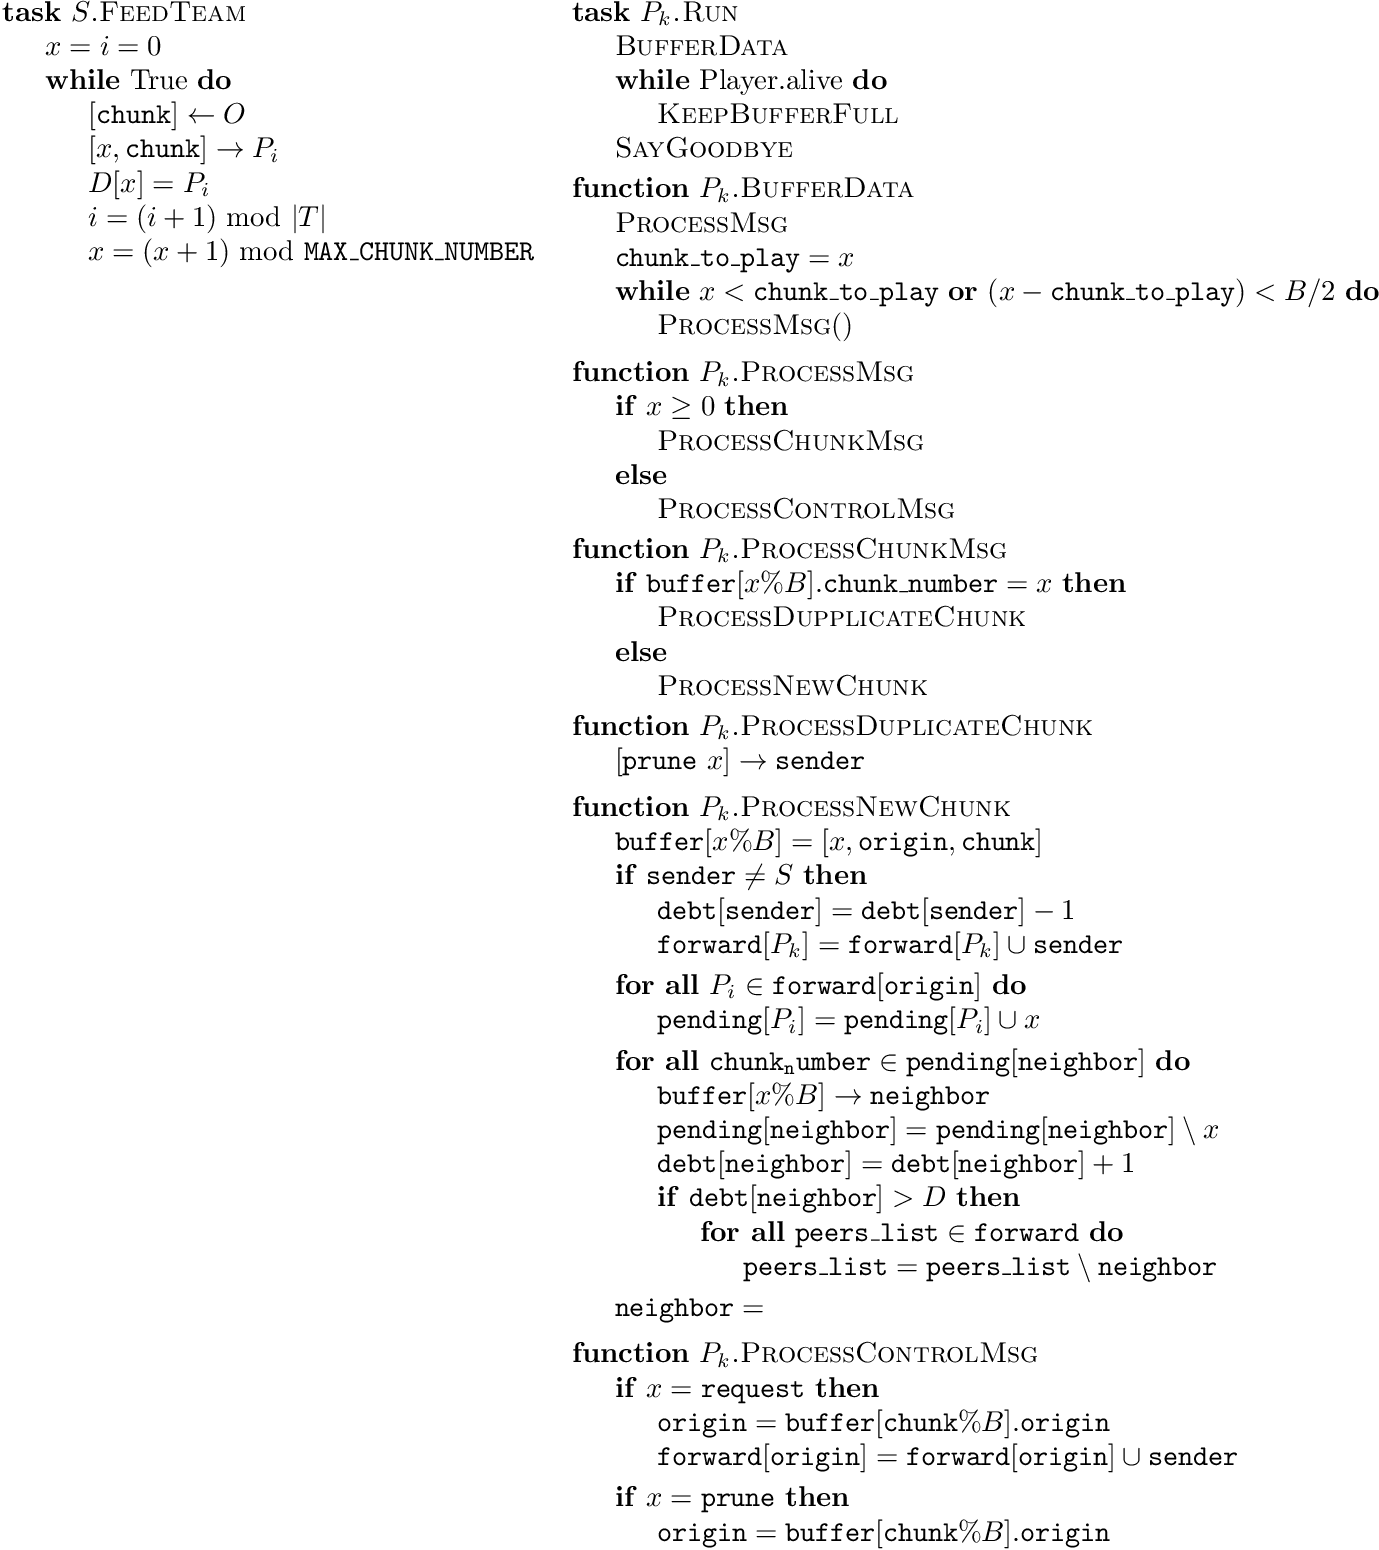
\includegraphics[width=0.75\textwidth]{chunk_generation_and_flooding}
  \fig{300}{chunk_generation_and_flooding}
  \caption{Chunk generation and
    flooding.\label{fig:chunk_generation_and_flooding}}
\end{figure*}
Each ${\cal S}_j\in{\cal S}$ (see
Fig.~\ref{fig:chunk_generation_and_flooding}) divides the stream into
chunks of data ($\mathtt{chunk}$) of constant length $C$ (and
identical content among teams), and sends exclusively each chunk to a
different \emph{origin peer} ${\cal P}_i\in{\cal T}_j$, using a
round-robin schema. Each chunk is enumerated with a index $x$, forming
the message $[c_x]=[x,\mathtt{chunk}]$, where
$x=i~\mathrm{mod}~|{\cal T}_j|$. We define a \emph{round} (in a team)
as the time necessary to send two consecutive chunks from the splitter
(of such team) to the same peer. This time is variable and depends on
$|{\cal T}_j|$, $C$, and the average bit-rate of the media, $R$.

\begin{comment}
The round-time is defined by:
\begin{equation}
  \cal{r} = \cal{c}N.
  \label{eq:round_time}
\end{equation}
For example, if we use only one team of $N=256$ peers, a chunk size
$C=1024$~bytes, and a video of $1$~Mb/s, the round time is
\begin{displaymath}
  \cal{r} = \frac{1024\frac{\text{bytes}}{\text{chunk}}\times
    8\frac{\text{bits}}{\text{byte}}}{10^6\frac{\text{bits}}{\text{second}}}\times
  256 \approx 2.1~\text{seconds}.
\end{displaymath}
\end{comment}
